\documentclass[11pt, a4paper]{article}
\usepackage{pdfpages}
\usepackage{parallel}
\usepackage[T2A]{fontenc}
\usepackage{ucs}
\usepackage[utf8x]{inputenc}
\usepackage[polish,english,russian]{babel}
\usepackage{hyperref}
\usepackage{rotating}
\usepackage[inner=2cm,top=1.8cm,outer=2cm,bottom=2.3cm,nohead]{geometry}
\usepackage{listings}
\usepackage{graphicx}
\usepackage{wrapfig}
\usepackage{longtable}
\usepackage{indentfirst}
\usepackage{array}
\usepackage{tikzsymbols}
\usepackage{soul}
\usepackage[ruled,vlined]{algorithm2e}
%\counterwithout{figure}{section} 

\usepackage{url}
\makeatletter
\g@addto@macro{\UrlBreaks}{\UrlOrds}
\makeatother

\newcolumntype{P}[1]{>{\raggedright\arraybackslash}p{#1}}
\frenchspacing
\usepackage{fixltx2e} %text sub- and superscripts
\usepackage{icomma} % коскі ў матэматычным рэжыме
\PreloadUnicodePage{4}

\newcommand{\longpage}{\enlargethispage{\baselineskip}}
\newcommand{\shortpage}{\enlargethispage{-\baselineskip}}

\def\switchlang#1{\expandafter\csname switchlang#1\endcsname}
\def\switchlangbe{
\let\saverefname=\refname%
\def\refname{Літаратура}%
\def\figurename{Іл.}%
}
\def\switchlangen{
\let\saverefname=\refname%
\def\refname{References}%
\def\figurename{Fig.}%
}
\def\switchlangru{
\let\saverefname=\refname%
\let\savefigurename=\figurename%
\def\refname{Литература}%
\def\figurename{Рис.}%
}

\hyphenation{admi-ni-stra-tive}
\hyphenation{ex-pe-ri-ence}
\hyphenation{fle-xi-bi-li-ty}
\hyphenation{Py-thon}
\hyphenation{ma-the-ma-ti-cal}
\hyphenation{re-ported}
\hyphenation{imp-le-menta-tions}
\hyphenation{pro-vides}
\hyphenation{en-gi-neering}
\hyphenation{com-pa-ti-bi-li-ty}
\hyphenation{im-pos-sible}
\hyphenation{desk-top}
\hyphenation{elec-tro-nic}
\hyphenation{com-pa-ny}
\hyphenation{de-ve-lop-ment}
\hyphenation{de-ve-loping}
\hyphenation{de-ve-lop}
\hyphenation{da-ta-ba-se}
\hyphenation{plat-forms}
\hyphenation{or-ga-ni-za-tion}
\hyphenation{pro-gramming}
\hyphenation{in-stru-ments}
\hyphenation{Li-nux}
\hyphenation{sour-ce}
\hyphenation{en-vi-ron-ment}
\hyphenation{Te-le-pathy}
\hyphenation{Li-nux-ov-ka}
\hyphenation{Open-BSD}
\hyphenation{Free-BSD}
\hyphenation{men-ti-on-ed}
\hyphenation{app-li-ca-tion}

\def\progref!#1!{\texttt{#1}}
\renewcommand{\arraystretch}{2} %Іначай формулы ў матрыцы зліпаюцца з лініямі
\usepackage{array}

\def\interview #1 (#2), #3, #4, #5\par{

\section[#1, #3, #4]{#1 -- #3, #4}
\def\qname{LVEE}
\def\aname{#1}
\def\q ##1\par{{\noindent \bf \qname: ##1 }\par}
\def\a{{\noindent \bf \aname: } \def\qname{L}\def\aname{#2}}
}

\def\interview* #1 (#2), #3, #4, #5\par{

\section*{#1\\{\small\rm #3, #4. #5}}
\ifx\ParallelWhichBox\undefined%
    \addcontentsline{toc}{section}{#1, #3, #4}%
\else%
\ifnum\ParallelWhichBox=0%
    \addcontentsline{toc}{section}{#1, #3, #4}%
\fi\fi%

\def\qname{LVEE}
\def\aname{#1}
\def\q ##1\par{{\noindent \bf \qname: ##1 }\par}
\def\a{{\noindent \bf \aname: } \def\qname{L}\def\aname{#2}}
}

\newcommand{\interviewfooter}[1]{
\vskip 1em
\noindent \textit{#1}
}

\switchlang{ru}
\begin{document}

\title{1989 "--- Fujitsu FM Towns model 1 mouse (FMT-MO101)}
\date{}
\maketitle
\selectlanguage{russian}

В феврале 1989 года компания Fujitsu анонсировала первую модель семейства компьютеров FM Towns, работавшую под управлением собственной графической системы Towns OS. FM Towns представляли собой проприетарный вариант компьютеров на основе PC-совместимой архитектуры, ориентированный на мультимедийные приложения и игры. Первая модель FM Towns была построена на базе процессора Intel 80386, оснащалась 1 или 2 Мб ОЗУ, приводом CD-ROM, микрофоном, геймпадом и мышью \cite{wikipedia}. C этой моделью поставлялась мышь FMT-MO101 (рис. \ref{fig:FMT1Pic}).

\begin{figure}[h]
    \centering
    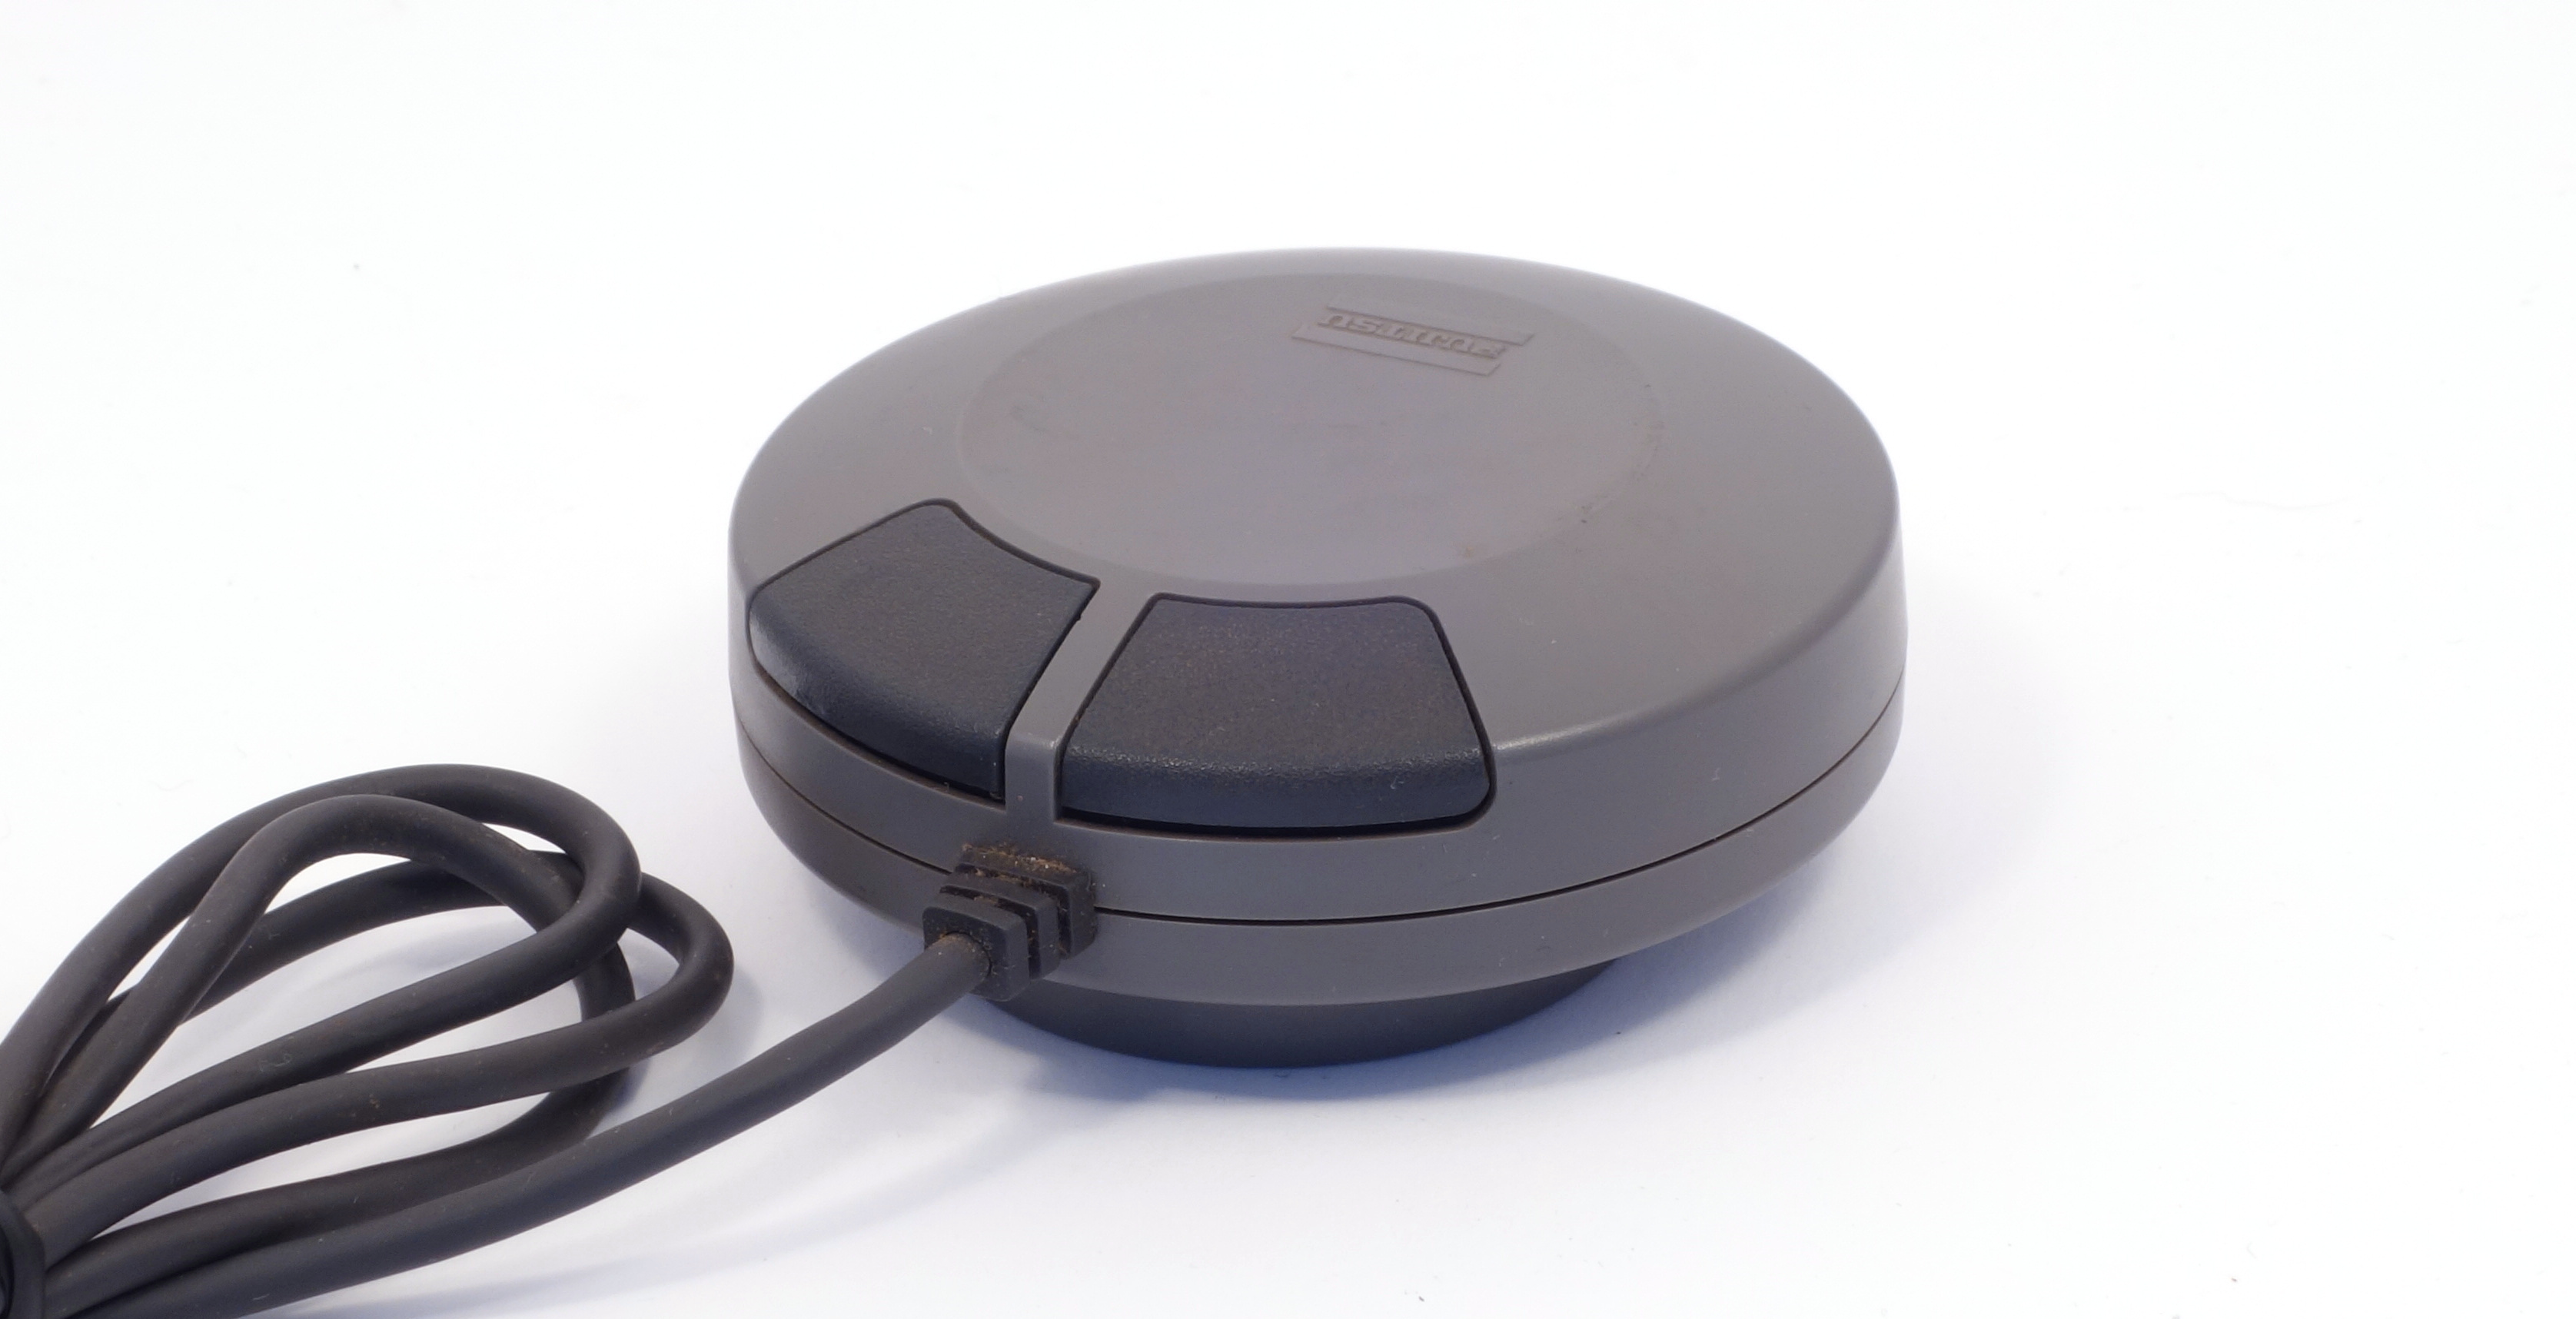
\includegraphics[scale=0.6]{1989_fujitsu_fmt_mo101_mouse/pic_30.jpg}
    \caption{Мышь Fujitsu FMT-MO101}
    \label{fig:FMT1Pic}
\end{figure}

Безусловно, главной особенностью этой мыши является ее круглая (а точнее, грибовидная) форма. Две достаточно крупные кнопки из более темной пластмассы в виде секторов расположены в передней части корпуса. Также с верхней стороны корпуса можно видеть рельефный логотип Fujitsu \cite{twinklemagic}. Нижняя часть мыши выглядит более традиционно, вклюая ножки из низкофрикционного материала и съемное кольцо-защелку, позволяющее извлечь шар для чистки. В целом дизайн корпуса определенно можно признать запоминающимся и эстетичным.

\begin{figure}[h]
    \centering
    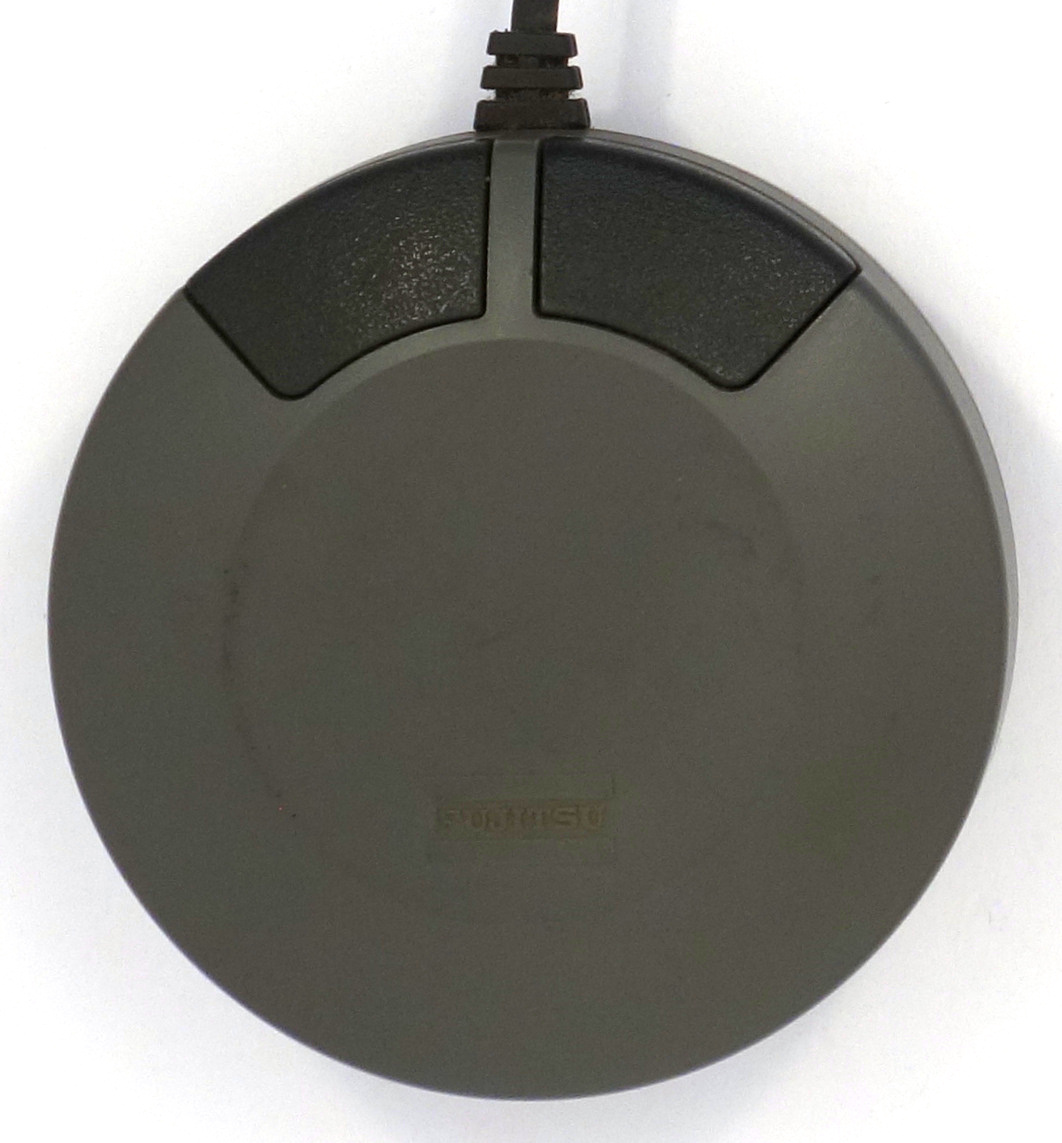
\includegraphics[scale=0.5]{1989_fujitsu_fmt_mo101_mouse/top_30.jpg}
    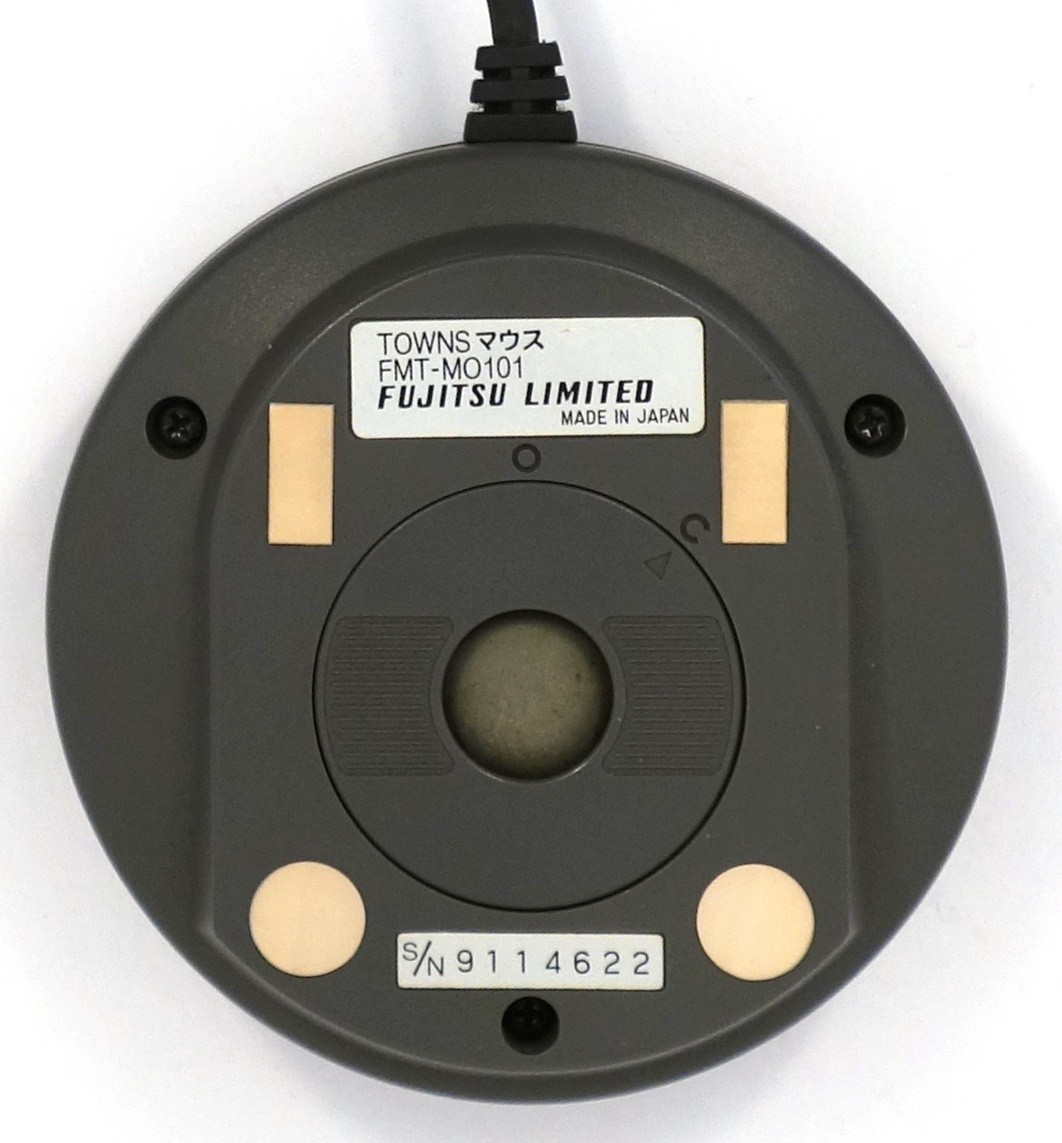
\includegraphics[scale=0.5]{1989_fujitsu_fmt_mo101_mouse/bottom_30.jpg}
    \caption{Мышь Fujitsu FMT-MO101, вид сверху и снизу}
    \label{fig:FMT1TopAndBottom}
\end{figure}

Мышь имеет средние размеры, что в сочетании с круглой формой делает ее слишком широкой \cite{twinklemagic} для удобного охвата ладонью (рис. \ref{fig:FMT1Size}, \ref{fig:FMT1Hand}).

\begin{figure}[h]
    \centering
    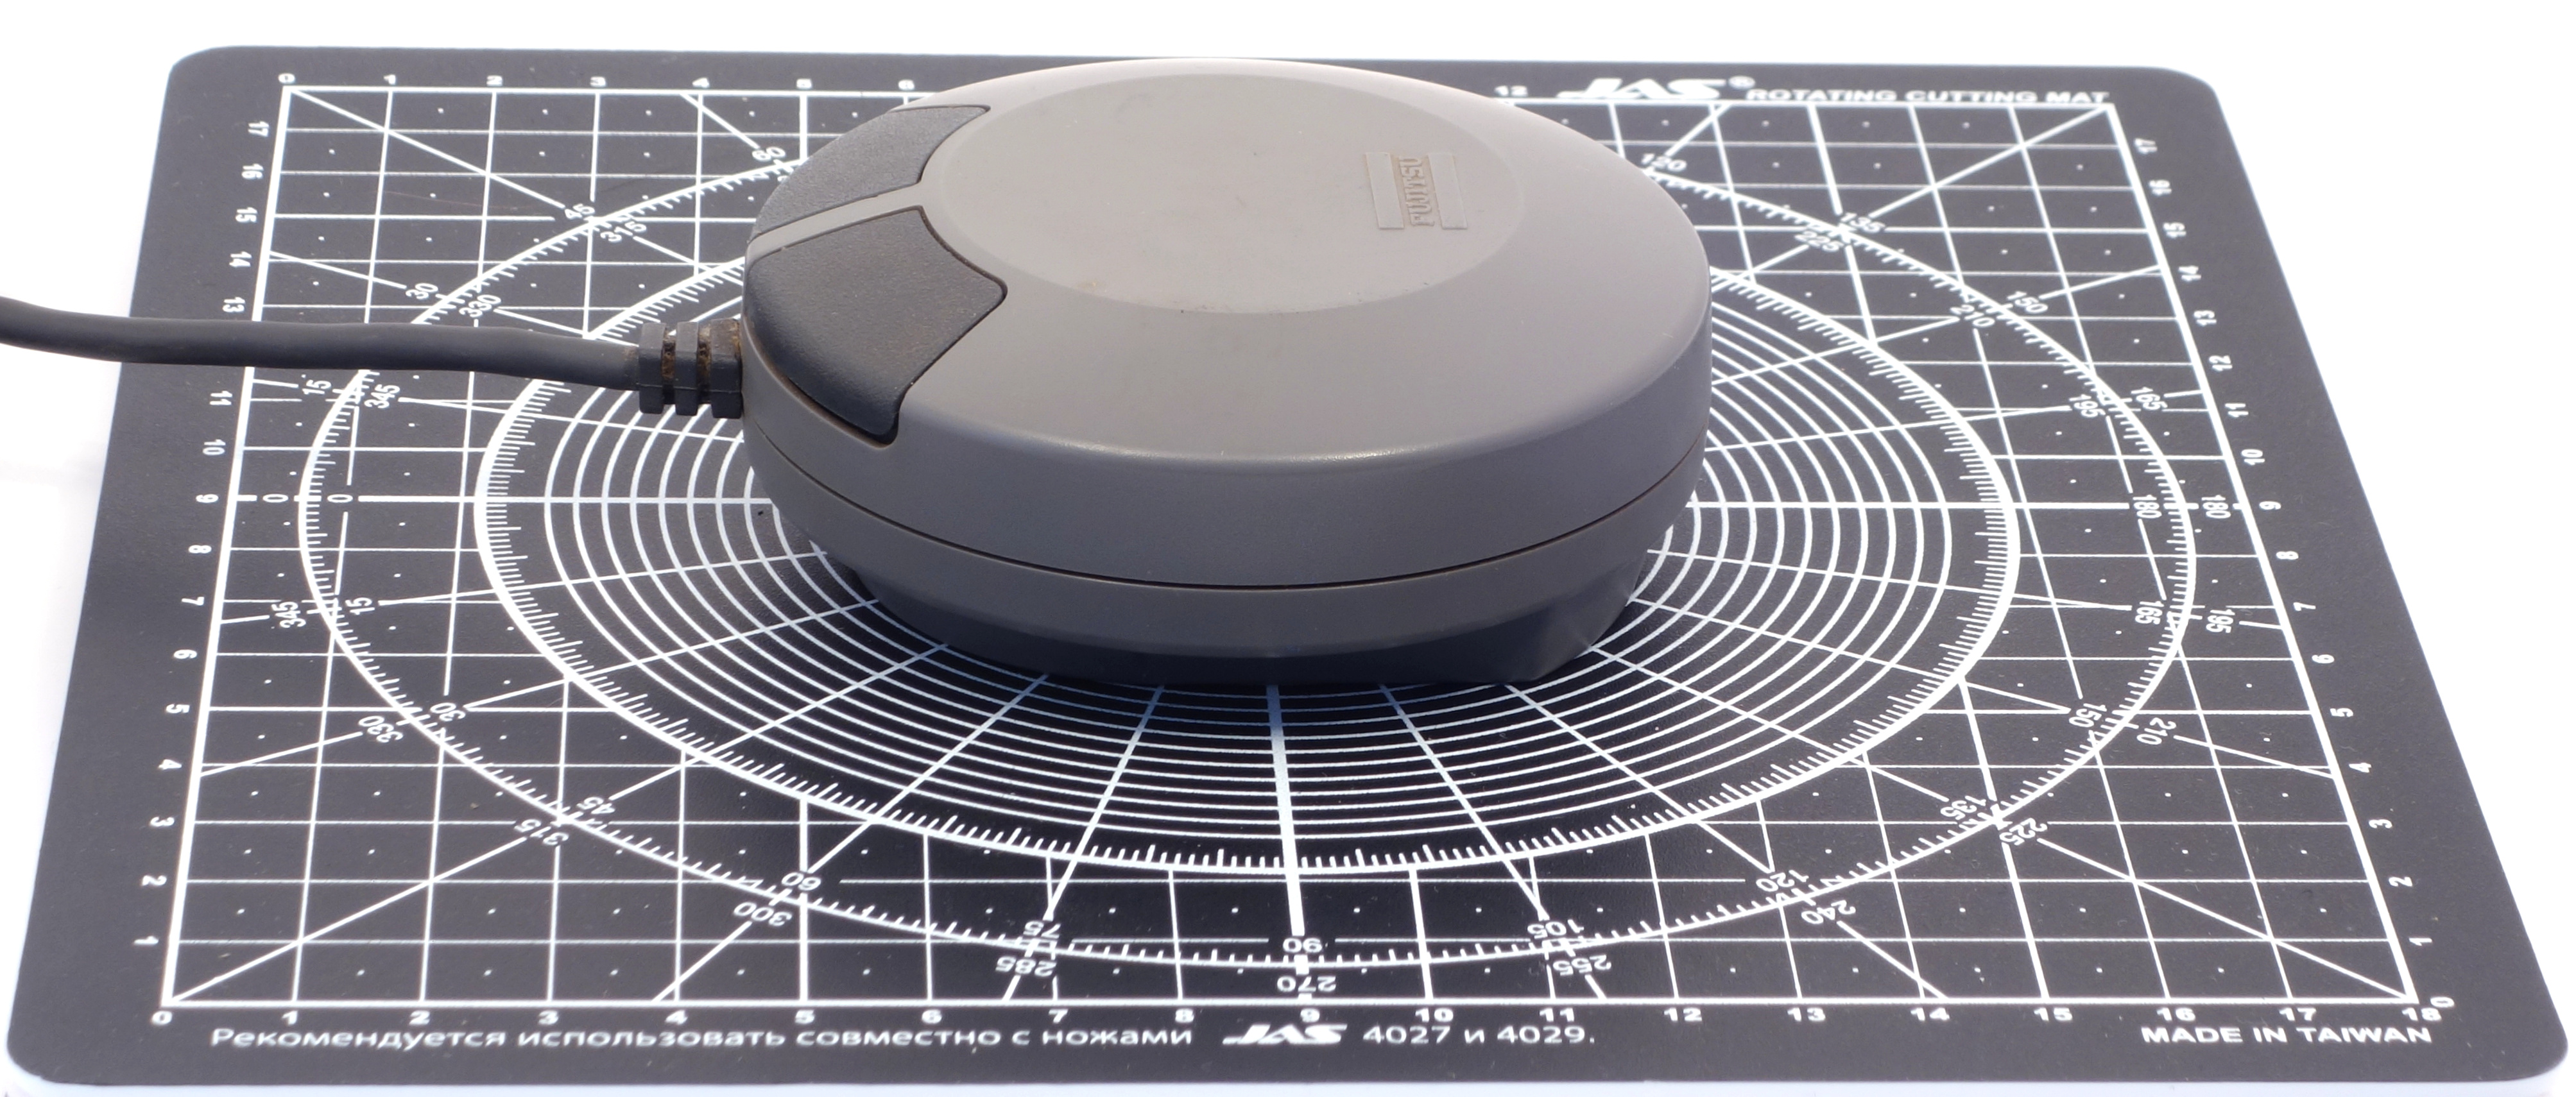
\includegraphics[scale=0.45]{1989_fujitsu_fmt_mo101_mouse/size_30.jpg}
    \caption{Мышь Fujitsu FMT-MO101 на размерном коврике с шагом сетки 1~см}
    \label{fig:FMT1Size}
\end{figure}

Очевидно также, что более узкое основание корпуса не добавляет мыши устойчивости. Эту проблему нельзя назвать сильно выраженной, но тем не менее пользователь инстинктивно старается меньше опираться на боковые края, чтобы ненароком не опрокинуть мышь. Очевидно по этой причине, последующие модели мышей для компьютеров FM Towns имели менее запоминающуюся но зато более практичную форму.

\begin{figure}[h]
    \centering
    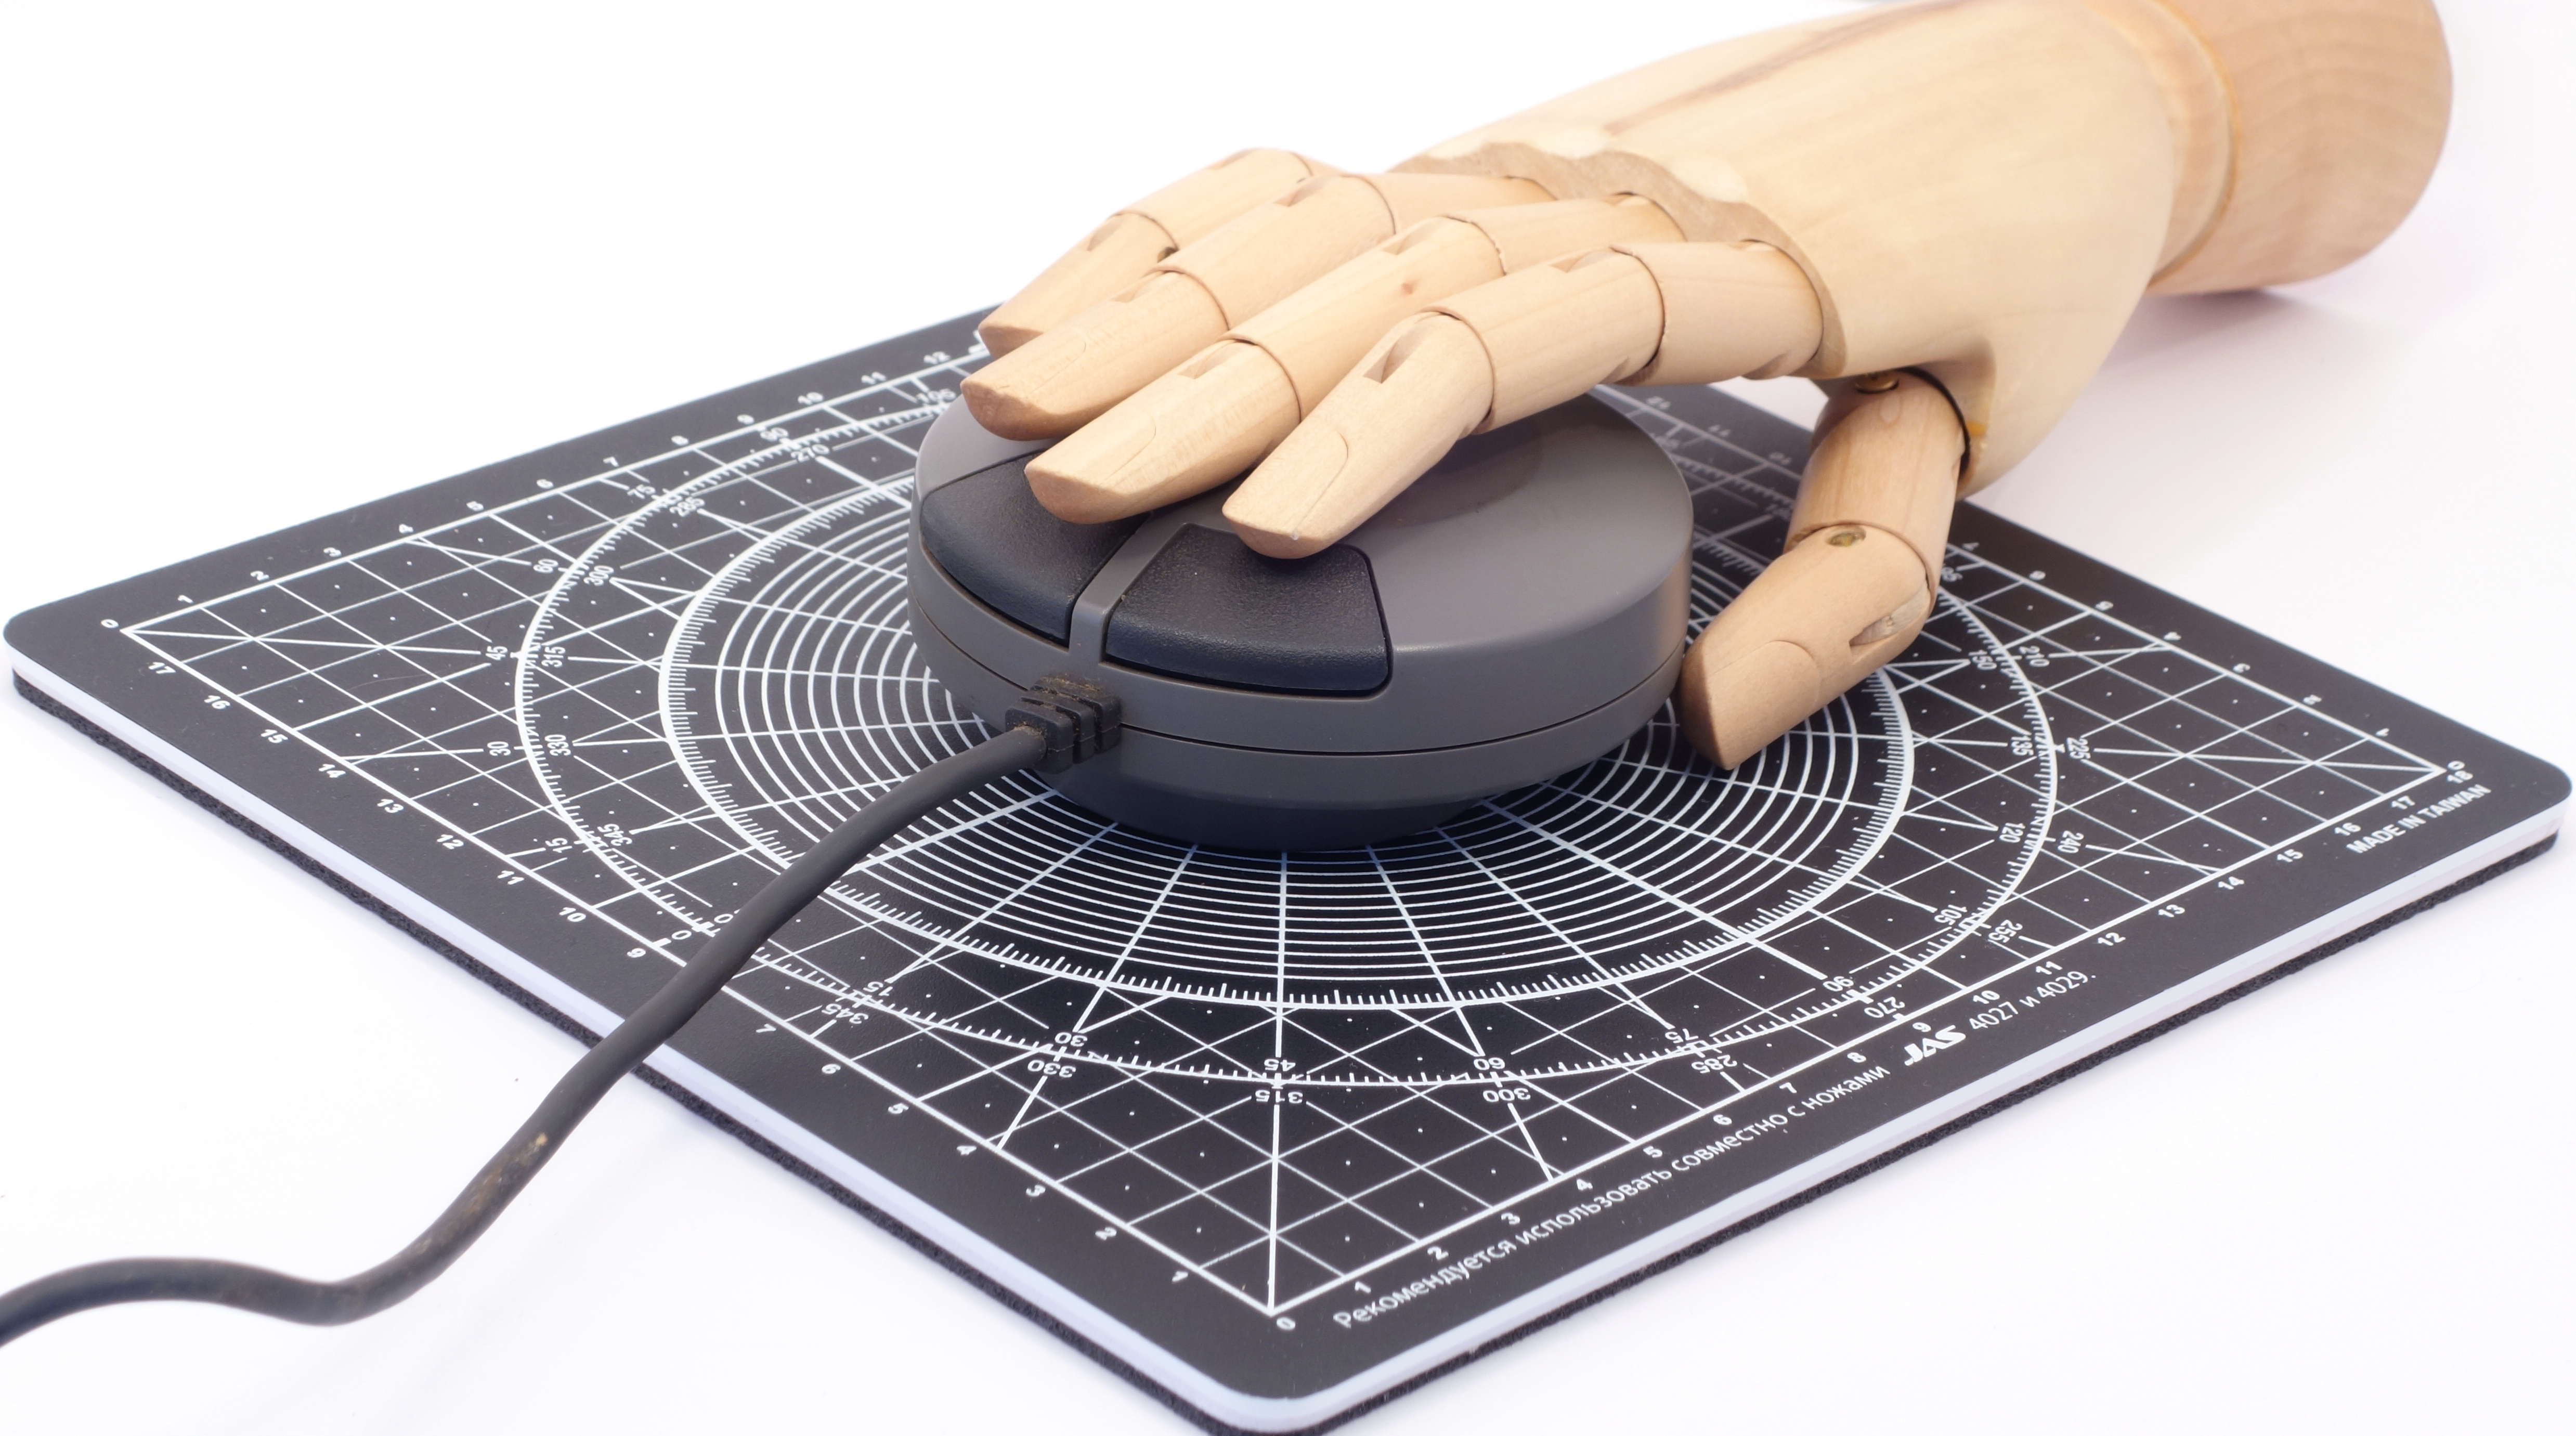
\includegraphics[scale=0.45]{1989_fujitsu_fmt_mo101_mouse/hand_30.jpg}
    \caption{Мышь Fujitsu FMT-MO101 с моделью руки человека}
    \label{fig:FMT1Hand}
\end{figure}

С технической точки зрения мышь FM Towns имеет интерфейс MSX, что делает ее достаточно универсальной в плане совместимости \cite{tepatti}.

Внутреннее устройство мыши показано на рис. \ref{fig:FMT1Inside}, что позволяет классифицировать  ее как оптомеханическую. Реализация является достаточно передовой для своего времени; при этом обращают на себя внимание металлические диски энкодеров, более типичные для дорогих мышей начала 80-х годов (например, мышей Depraz).

\begin{figure}[h]
    \centering
    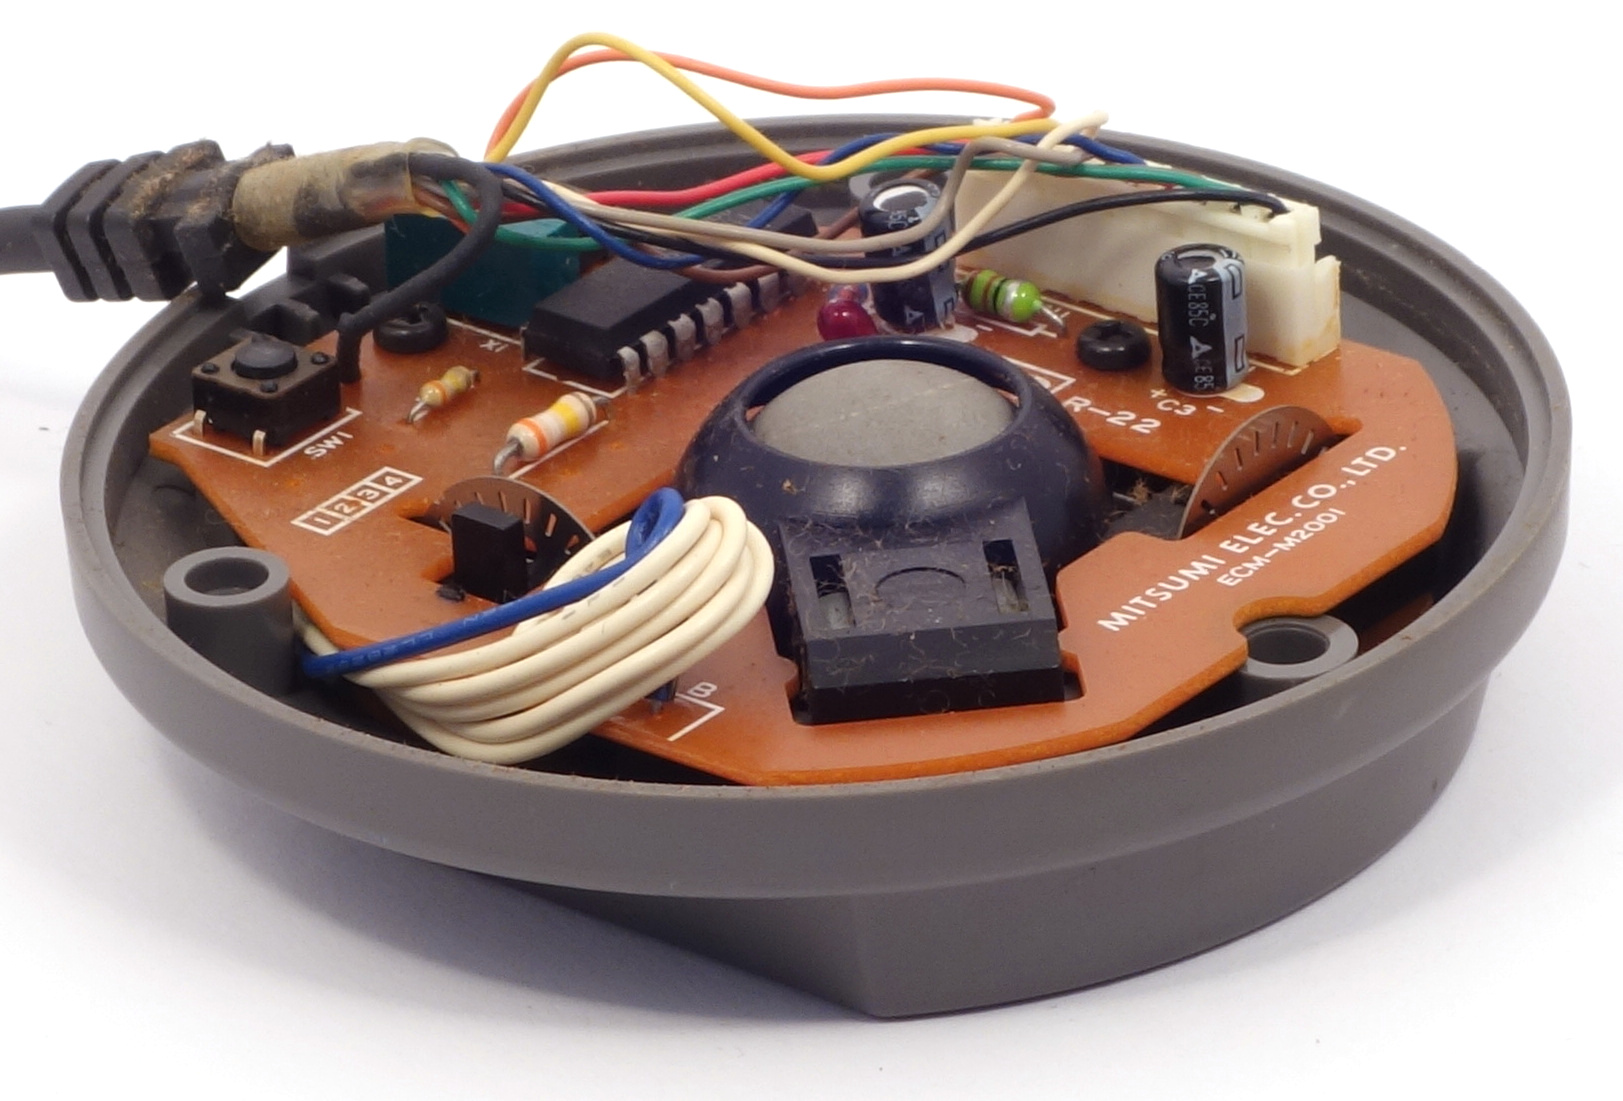
\includegraphics[scale=0.8]{1989_fujitsu_fmt_mo101_mouse/inside_30.jpg}
    \caption{Мышь Fujitsu FMT-MO101 в разобранном виде}
    \label{fig:FMT1Inside}
\end{figure}

\begin{thebibliography}{9}
    \bibitem{wikipedia} FM Towns \url{https://en.wikipedia.org/wiki/FM_Towns}
    \bibitem{twinklemagic} Mouse to mouse \url{http://twinklemagic.la.coocan.jp/towns/mouse/MOUSE_to_MOUSE.html} 
    \bibitem{tepatti} Tepatti T. FM Towns Keyboards, Mice, and Game Pads \url{https://tepatti.com/blog/005/index.html}
\end{thebibliography}

\end{document}
